\documentclass[conference]{IEEEtran}
\IEEEoverridecommandlockouts
% The preceding line is only needed to identify funding in the first footnote. If that is unneeded, please comment it out.
\usepackage{cite}
\usepackage{hyperref}
\usepackage{amsmath,amssymb,amsfonts}
\usepackage{algorithmic}
\usepackage{listings}
\usepackage{graphicx}
\usepackage{textcomp}
\usepackage{xcolor}
\def\BibTeX{{\rm B\kern-.05em{\sc i\kern-.025em b}\kern-.08em
    T\kern-.1667em\lower.7ex\hbox{E}\kern-.125emX}}
    
\begin{document}

\title{Developing a Domain Specific Language for visualizing geospatial data}

\author{
\IEEEauthorblockN{ Christopher Stelzmüller}
\IEEEauthorblockA{Domain Specific Languages, Topic 2 \\
11814096 / 521\\
c.stelzmueller@triply.at}
\and
\IEEEauthorblockN{ Sebastian Tanzer}
\IEEEauthorblockA{Domain Specific Languages, Topic 2 \\
11826853 / 521\\
s.tanzer@triply.at}
}

\maketitle

\begin{abstract}
The application of geospatial big data to an increasing number of topics presents new opportunities and challenges for cartographic researchers. Many emerging technologies focus on providing functionality to implement appealing and informative visualisations. At the same time, most web-based geospatial data visualisation technologies rely on simple configuration files for defining styling. We propose a type-safe domain-specific language for implementing reusable map visualisations with MapboxGL to improve development efficiency and utilise IDE support.
\end{abstract}

\begin{IEEEkeywords}
data visualization, mapbox, domain specific language, geospatial, big data
\end{IEEEkeywords}

\section{Introduction}
\IEEEPARstart{W}{ith} the advent of more and more practical opportunities for geospatial data applications in multiple new domains, the need for implementing geospatial visualization in an efficient and dynamic way is increasing. Visualizations are no longer only accessed from desktop computers, but rather viewed from a multitude of different devices. 
At the same time, the rise of augmented- and virtual reality capabilities in everyday devices is providing a vast array of new possibilities in visualizations and has increased the demand for more interactivity. 

Based on these recent developments, more and more cartographic researchers have switched from creating graphics in traditional geographic information system (GIS) software to creating interactive visualizations using web-based map frameworks. 
One of said web-based map frameworks is Mapbox GL. Besides providing sophisticated tools for designing map styles interactively\cite{dunn2017custom}, Mapbox also provides software development kits for including their maps in augmented- and virtual reality applications developed with the Unity framework.
Furthermore, Mapbox uses a shared style language for designing maps for both native and web-based viewing in mobile and desktop applications.

The appearance of  Mapbox GL JS map visualizations is defined by the \textit{Mapbox GL JS style specification} (MS specification). By using a specific JSON document that consists of a root object with multiple child nodes different properties of the map visualization can be set \cite{mapbox2020style}.

Even though the MS specification is generally intuitively designed and easy to understand, defining styles with a JSON configuration file comes with a diverse set of problems. 
The most apparent problem is the lack of static analysis tooling and editor support, which prevents problems and bugs from being recognized at compile-time. 

In this paper we want to highlight the problems and potential pitfalls of developing map visualizations with \textit{Mapbox style specification} and show how they could be mitigated by implementing a domain specific language for visualizing geospatial data. 

For the purpose of showing said problems, we will implement a visualization for the following practical use-case: We want to display Vienna's population distribution in a three-dimensional map. Figure \ref{fig:map_viz} shows an exemplary visualization of the aforementioned data. 

\begin{figure}
    \centering
    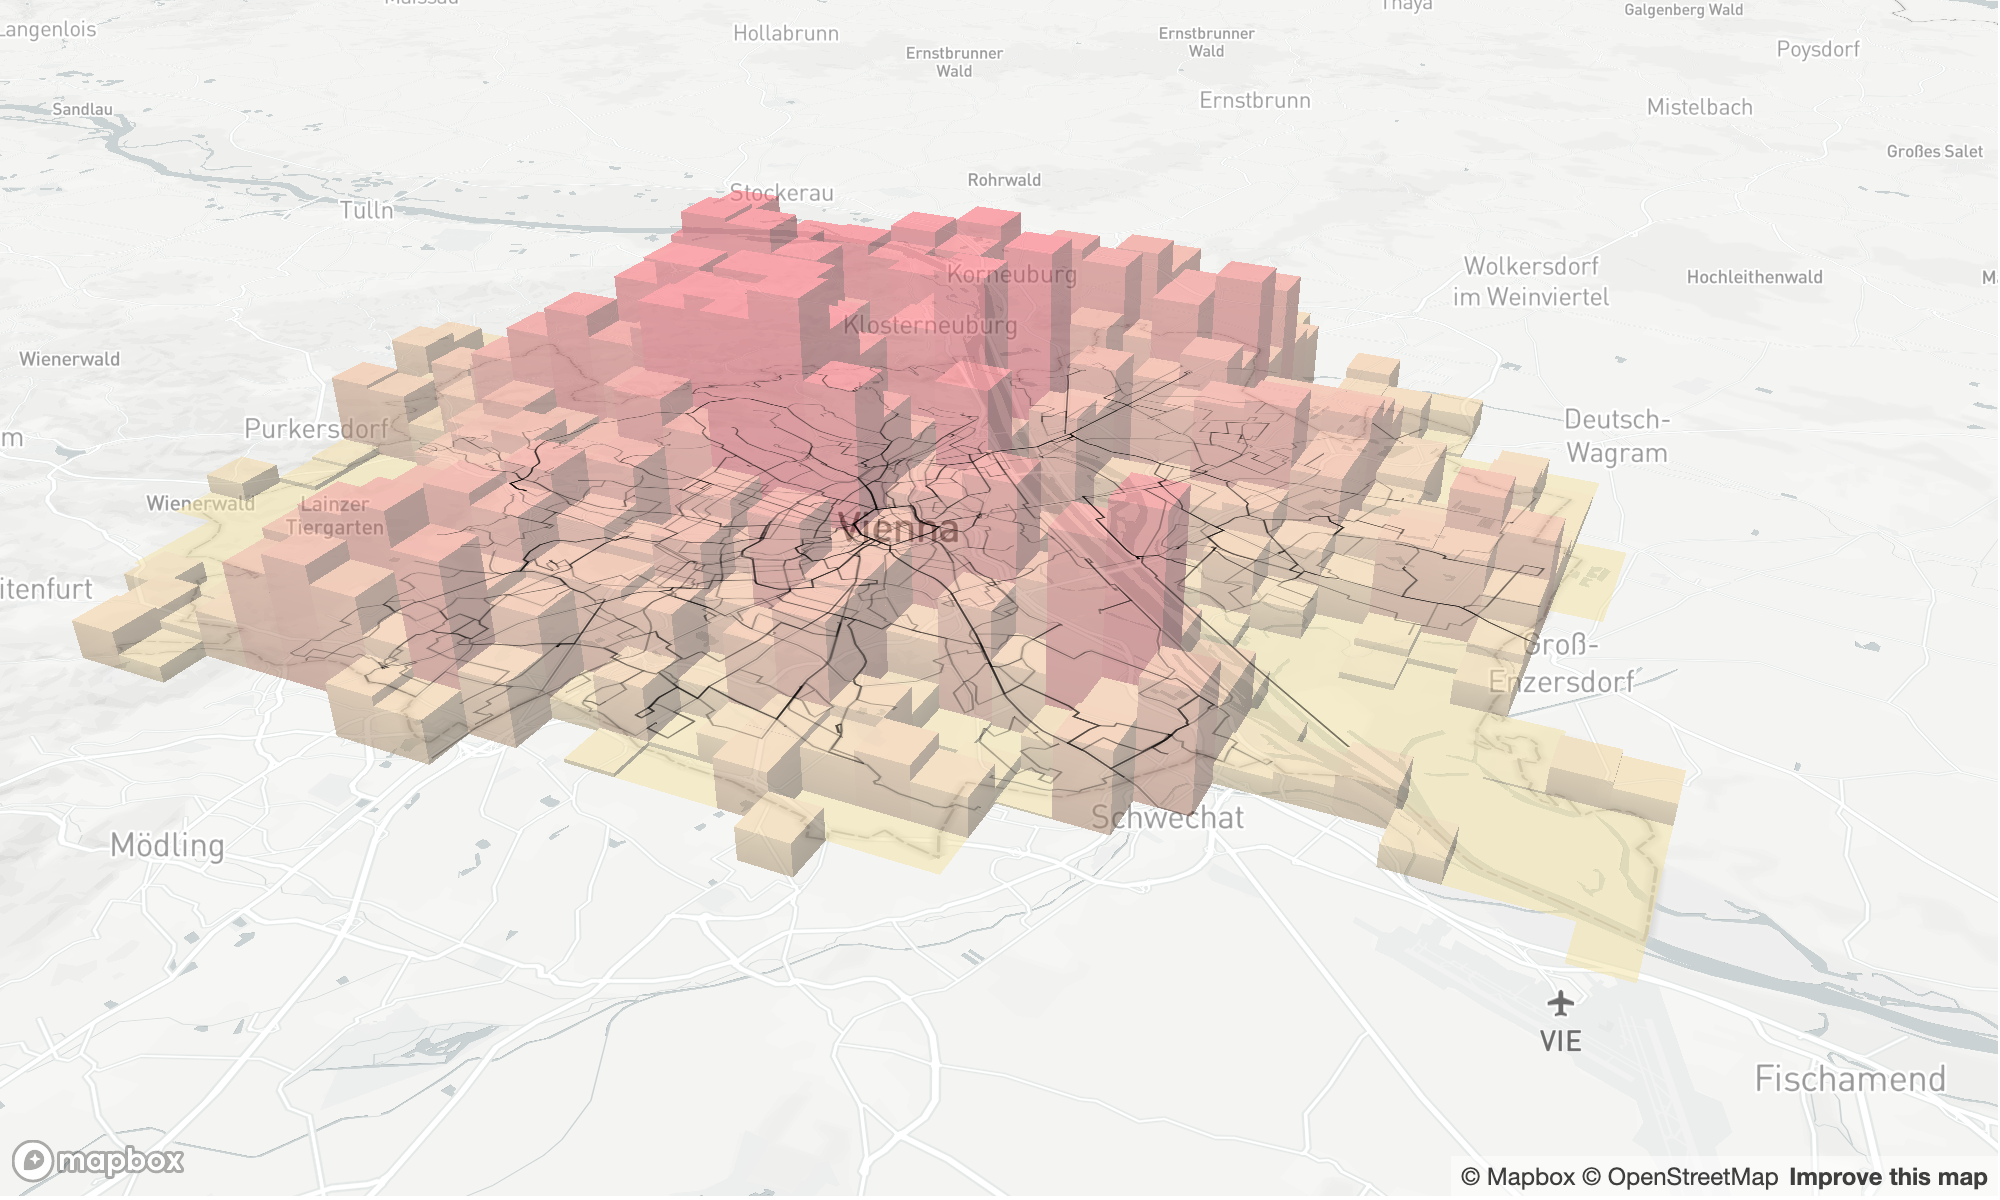
\includegraphics[width=\columnwidth]{img/population_vienna.png}
    \caption{Exemplary visualization: Population in Vienna}
    \label{fig:map_viz}
\end{figure}

\section{Background and Related Work}
Kuhn et al \cite{kuhn2015designing} discuss the viability of implementing a high-level language for the domain of Spatial Computing, identify the core concepts of spatial information underlying spatial computing and present a first draft of their language in an exemplary python implementation.

Alvarado et al \cite{alvarado2019dsl} define a domain specific language to automatically generate GIS applications that include the most common components. The aim of their DSL is not to create a fully-featured and finalized GIS product from scratch, but rather to automatically generate a  system which serves as the basis for further development and customization.

GIScript is a domain specific language that was proposed by Zhang et al \cite{zhang2014gis} and identifies parallel execution and good interoperability as its main concerns. The proposed exemplary implementation is built on Python and uses \textit{Parallel Python} for parallel processing of tasks. GIScript scripts should be able to be executed by Open Source GIS software that allow python scripting as for instance QGis and GRASS GIS do.

\subsection{Mapbox GL}

A MSS JSON configuration consists of a root object which contains properties that change the appearance of the whole map. Most commonly, the following values, objects and arrays are configured: 

\begin{enumerate}
    \item \textbf{sprite:} (string): a link to the base style of the map underlying the visualization
    \item \textbf{center:} (array of number) the center of the map
    \item \textbf{bearing:} (number) the angle by which the map is rotated
    \item \textbf{sources:} (object with \textit{Source} values) data sources for the visualization
    \item \textbf{layers:} (array of \textit{Layer} values) layers in the visualization, in the order that they should be drawn
\end{enumerate}

Since GeoJSON is widely used, is one of the de-facto standards for spatial vector data and can be easily converted to and from other spatial data-formats\cite{dixson2020geojson}, we will focus on visualizing GeoJSON data layers in Mapbox GL JS.

A very useful feature of MSS is the ability to use \textit{data expressions} in order to dynamically apply properties and values from a data source to the map visualization. Expressions can be used to specify layout, paint or filter properties in layers. Each expression generally has the following structure: 
\\
\lstinline{[expression, arg0, arg1, ...]}
\\
Assuming the referenced data source contains an integer property \textit{population}, the expression in figure \ref{fig:exp1} can be used to scale a circle's size with the population of the according feature. While this syntax allows for short and expressive expression definitions, expressing nested and more complicated constructs can lead to very big, and by extension also confusing expressions.

\begin{figure}
    \centering
    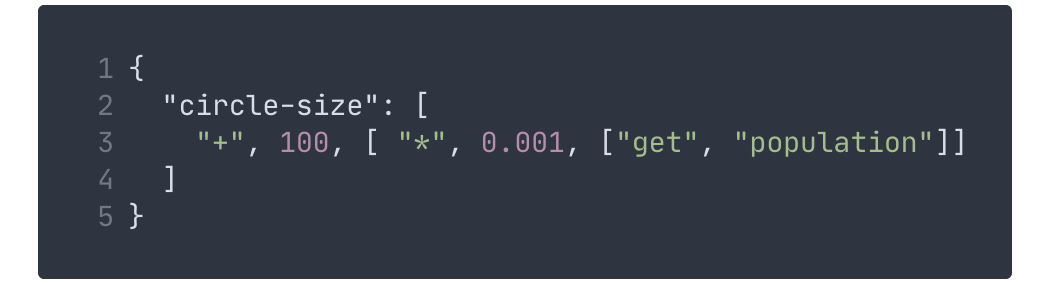
\includegraphics[width=\columnwidth]{img/circlesize.png}
    \caption{Scaling circle-size with data expression}
    \label{fig:exp1}
\end{figure}

% TODO: if there's too much empty space, we can add a comparison between e.g. mapbox and google maps here 
% \subsubsection{comparison to other mapping frameworks}
% - uses webgl for map rendering

% - very customizable

% - useful for data visualizations

% - styles from style language or designed in mapbox-studio

\subsection{Domain Specific Languages}

The idea behind a Domain-Specific Language (DSL) is a customised high-level abstraction language to a particular problem and domain, with the aim of providing a much better solution for the particular problem rather than a general-purpose language does\cite{van2000domain}.


DSLs can be categorised into two main types, namely  external DSL and internal DSL (also called embedded DSL).  
\\
An internal DSL is an extension to an existing General-Programming Language (GPL). It uses only parts of the syntactic elements
of the underlying language for a specific task of the overall system\cite{fowler2010domain}. 
\\
An external DSL is separated from the main language and defined in a different format. It can either have a custom syntax or uses the syntax of another language\cite{zdun2010dsl}.

Regardless of it's type, most DSL's commonly provide the following advantages to developers, designers, and it's users:

\subsubsection{Improving Productivity}
By providing notations and constructs for a specific application domain, DSLs provide ease of use compared with GPLs in a certain domain and increase productivity\cite{10.1145/1118890.1118892}. A DSL provides means to make code more readable and makes it easier to specify the intend in an understanding way. As a result, the time needed to investigate and fix mistakes is reduced and modifying a system gets also easier. Which again leads to an increase in productivity.
\subsubsection{Editor-Support and Validation}
For a subset of DSLs, another benefit is the possibility to provide custom syntax, check for elements and provide custom error messages. This ability allows for much safer and easier use for non-technical stakeholders.
\subsubsection{Accessibility and Communication}
By reducing the complexity of code and amount of required programming expertise compared to GPLs, DSLs are also more accessible by a larger group of developers. This enables better communication channels between programmers, customers and users of software and can even help to enable business domain experts to engage in the development of business information systems\cite{aram2015multilayered}.

\subsubsection{Reusablilty}
Especially for the construction of large software systems, but also in general one advantage of DSLs is that it enables the reuse of software artefacts, like source code, software design, domain abstractions and language grammars. An example is the implementation of a DSL as an application library, which clearly enables reuse of source code\cite{mernik2005and}.

\section{A DSL for Mapbox Styles}

\begin{figure}
    \centering
    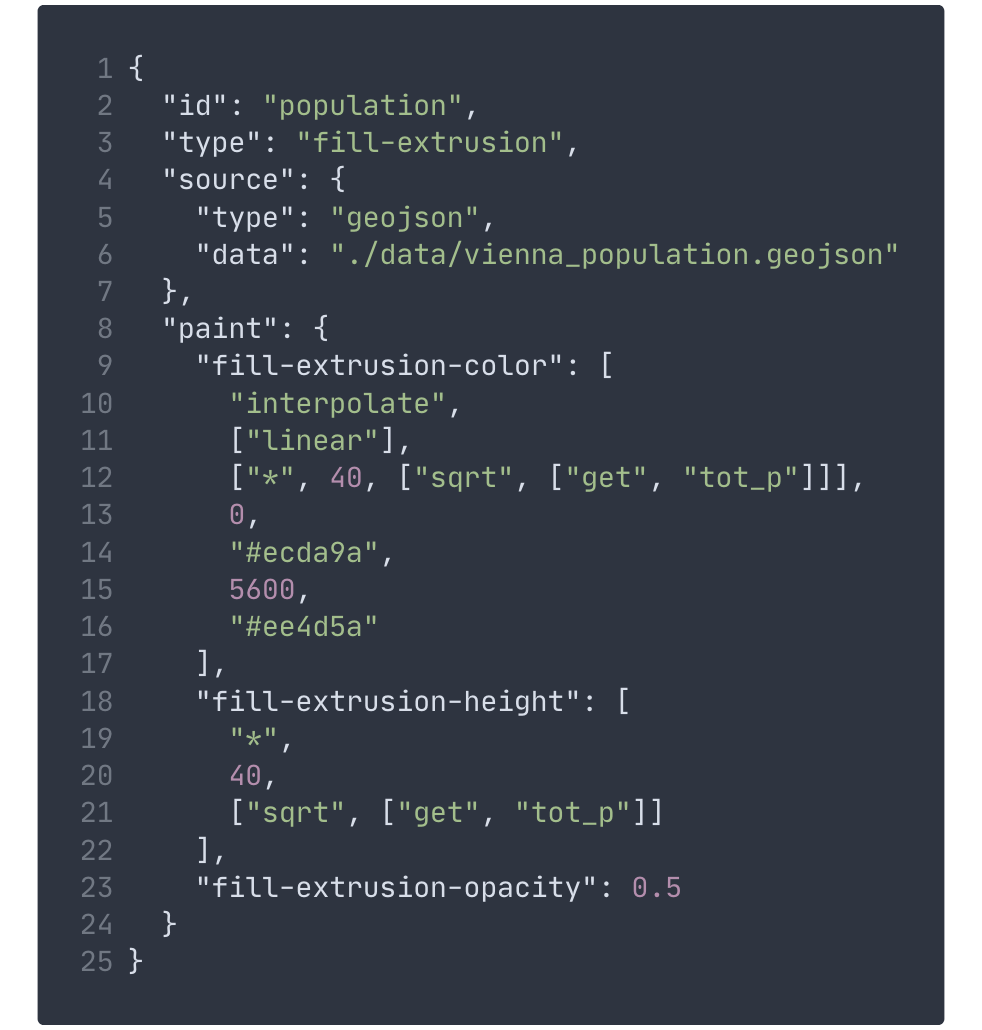
\includegraphics[width=\columnwidth]{img/vienna-mapbox.png}
    \caption{Layer configuration for population layer}
    \label{fig:mapbox-config}
\end{figure}
% page 3 - 3.3
To implement the 3D-elevation component of the visualization in figure \ref{fig:map_viz} the layer configuration specified in figure \ref{fig:mapbox-config} was used. This quick example illustrates a few of the problems that can come up when implementing visualizations with Mapbox GL JS. 

First up, there is yet no static analysis tool that can be used in IDEs during the development process. This means, that developers have to run their code in order to see if all properties are specified correctly and generally makes the code more prone to errors. 
In simple examples this is often not a problem, but when applications get more and more complex, validating if all possible states of an application can become challenging. 

Furthermore, Mapbox GL's internal configuration validation has the bad habit of sometimes being failing silently. This is best illustrated by a short example: The layer specified in figure \ref{fig:mapbox-config} is a \textit{fill-extrusion} layer, therefore the layer's paint properties have to be specified with the \textit{fill-extrusion} prefix\cite{mapbox2020style}. 
Due to the nature of how Mapbox GL parses the configuration objects, paint properties that are wrongly specified with a wrong prefix (e.g. \textit{fill-color}) are ignored completely and the default values are used. Even though this behaviour is according to the style specification, debug hints or warnings would be beneficial to developers.

Generally speaking, the lack of static analysis tools and the tendency to silent failures do not yet justify the development a domain specific language for the task at hand. Both these problems generally originate from the usage of JSON configuration files, and luckily there also exists a solution for them that originates from the JSON ecosystem. By defining the structure of the configuration objects via a JSON-schema, both syntactical structure and semantics of configurations could be validated statically\cite{pezoa2016json}.

Last but not least, layer configurations right now do not have any kind of IDE support. Providing better IDE support for developing visualizations would not only allow faster development speed and easier access to documentation, but could also help prevent errors and simplify changing parts of the visualization. Unfortunately, providing sophisticated IDE support for the existing configuration-file based code is not easily possible. 

In order to overcome this limitation and improve the general developer experience and velocity when developing Mapbox GL visualizations we propose a domain specific language for Mapbox Styles.


\subsection{Different approaches and tools for developing DSLs}
When creating domain-specific languages, several tools can be used to do so. A few examples are Rascal, a  language for meta-programming and the intend to solve problems in the domain of source code analysis and transformation\cite{klint2009easy}.
GMF (Graphical Modelling Framework) a java-based graphical editor in the form of an eclipse plugin that provides the infrastructure to create, from a UML like model\cite{james2011designing}.
JetBrains MPS (Meta Programming System), is an open-source language workbench developed by Jetbrains. A central feature of MPS is its projectional editor, which is one style of implementing the core of a language workbench\cite{voelter2019lessons}.

Another approach is to build the DSL based on an existing language inheriting its infrastructure and tailoring it in a unique way to the domain of interest, resulting in a domain-specific embedded language. This approach does not require the development of a new language for scratch and still facilitates an infrastructure that allows reuse of syntax, semantics, implementation code and other related artefacts\cite{685738}.
 
\subsection{Implementation}
One of the most important aspects for choosing which toolkit and programming language to implement the DSL is interoperability with the existing tool-sets already present. Since, in this paper we focus mostly on creating web-based visualizations, the most important topic of interoperability was to easily be included in JavaScript front-end code. This narrows down our choice of languages to languages that either run natively (e.g. JavaScript) or can be transpiled to languages that run natively in the browser (e.g. kotlin and Typescript).

Of the aforementioned languages, kotlin is the only one that not only can be transpiled to JavaScript for running in web-based projects, but can also be compiled to both JVM and native code. This also allows utilising the developed DSL for implement visualizations as a part of mobile or desktop applications. Regardless of these benefits, this paper will solely focus on developing an exemplary implementation for web-based visualizations.

The code for creating the population layer needed for the visualization in figure \ref{fig:map_viz} using our exemplary implementation of the MapboxDsl in kotlin is shown in figure \ref{fig:dsl-config}. We can see that by utilizing the proposed DSL, the required code is not only becoming more concise and readable at the same time, but can also be statically validated: An IDE is now able to highlight errors and problems with both expressions and value declarations before the code has been executed.

An additional benefit is the better development experience when implementing configurations with MapboxDsl. This benefit stems in equal parts from the ability to use \textit{KDoc} comments to provide additional documentation in the place where the code is used and the possibility to get IDE-provided suggestions and completions while writing code. \textit{KDoc} is the documentation style of the kotlin language and is syntactically similar to the \textit{JavaDoc} commenting style. 
By providing comments in the specified format extensive documentation, development hints and usage examples can be defined. By utilising IDE support, this additional information can then be shown to developer without having to first navigate through external documentation. Another - in this case very helpful - feature of \textit{KDoc} is the ability to specify documents in the Markdown format which brings the helpful ability to include images in documentation code for  style definitions.

\begin{figure}
    \centering
    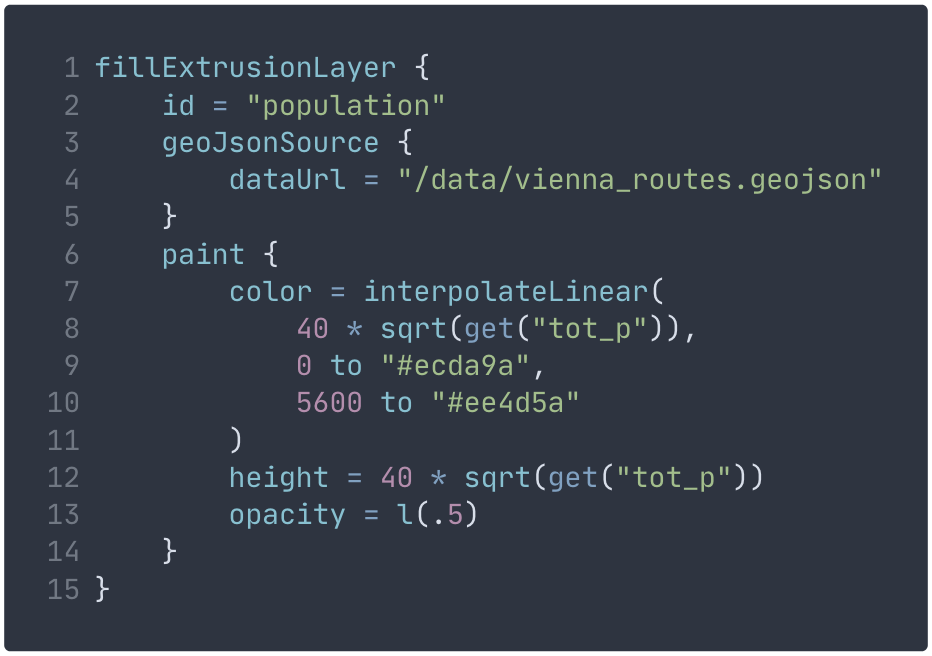
\includegraphics[width=\columnwidth]{img/vienna-dsl.png}
    \caption{Layer configuration for population layer with MapboxDsl}
    \label{fig:dsl-config}
\end{figure}

\section{Conclusion and future work}

Spatial data visualization is a task that requires both modern technologies, fast development speed and short turn-around times when it comes to providing up-to-date visualizations on current topics. Due to these reasons, the field of spatial data visualization profits greatly from the implementation of a domain specific language that simplifies authoring web-based geospatial data visualizations.

In this paper, we have proposed an exemplary implementation of the MapboxDsl using the kotlin programming language. Furthermore, we have shown the viability of implementing a DSL for the topic at hand by comparing alternative solutions for solving problems related to configuration files used by Mapbox to our proposed solution. Last but not least, we have shown the differences and advantages of using a DSL for defining visualisations compared to regular JSON configuration files in a practical use-case.

As of now, our proposed exemplary implementation of MapboxDsl only contains the functionality for creating the map visualization shown in figure \ref{fig:map_viz}. To not only cover our exemplary use-case the remaining parts of the Mapbox GL Style Specification also have to be added to MapboxDsl. 

Future work includes implementing the remaining features, as specified in the MS specification. Futhermore, MapboxDsl should be able to be adapted for usage on the Android, iOs and Unity platforms as well, in order simplify generating map visualizations on all platforms supported by Mapbox.


\section*{Acknowledgment}

All data and example code used in this paper can be found in the github repository at  \href{https://github.com/tuesd4y/mapbox-dsl}{https://github.com/tuesd4y/mapbox-dsl}.

TODO.. ideas: 

This work has been supported by as company?.

We particularly want to thank \textit{somebody?} for their feedback and support. Special thanks go to coffee for keeping us energized to finish in time.

\bibliographystyle{plain} % We choose the "plain" reference style
\bibliography{refs.bib} % 

\end{document}
